	El núcleo del Kit de Desarrollo FX2LP EZ-USB es un CY7C68013A. Dicho circuito integrado, cuya arquitectura se presenta en la Figura \ref{arqEzUSB}, pertenece a la serie FX2LP de la familia de integrados EZ-USB comercializado por Cypress Semiconductors. Esta serie se caracteriza por brindar una conexión USB 2.0 de alta velocidad y bajo consumo energético, especialmente diseñados para productos con autonomía limitada.\\
	
	Esta serie integra un controlador USB completo, incluyendo un transceptor USB, un MIS (Motor de Interfaz Serial), buffers de datos implementados con memorias tipo FIFO (\(First In First Out\); Primero Entrado, Primero Salido), un microcontrolador 8051 mejorado y una interfaz programable hacia los periféricos. Además posee un un PLL y un divisor configurable a través de los cuales provee al sistema de las señales de reloj adecuadas para el correcto funcionamiento del sistema.\\
	
	\begin{figure}[h]
		\centering
		%TODO meter la imagen
%		\includegraphics[width=.7\textwidth]{arqfx2lp.png}
		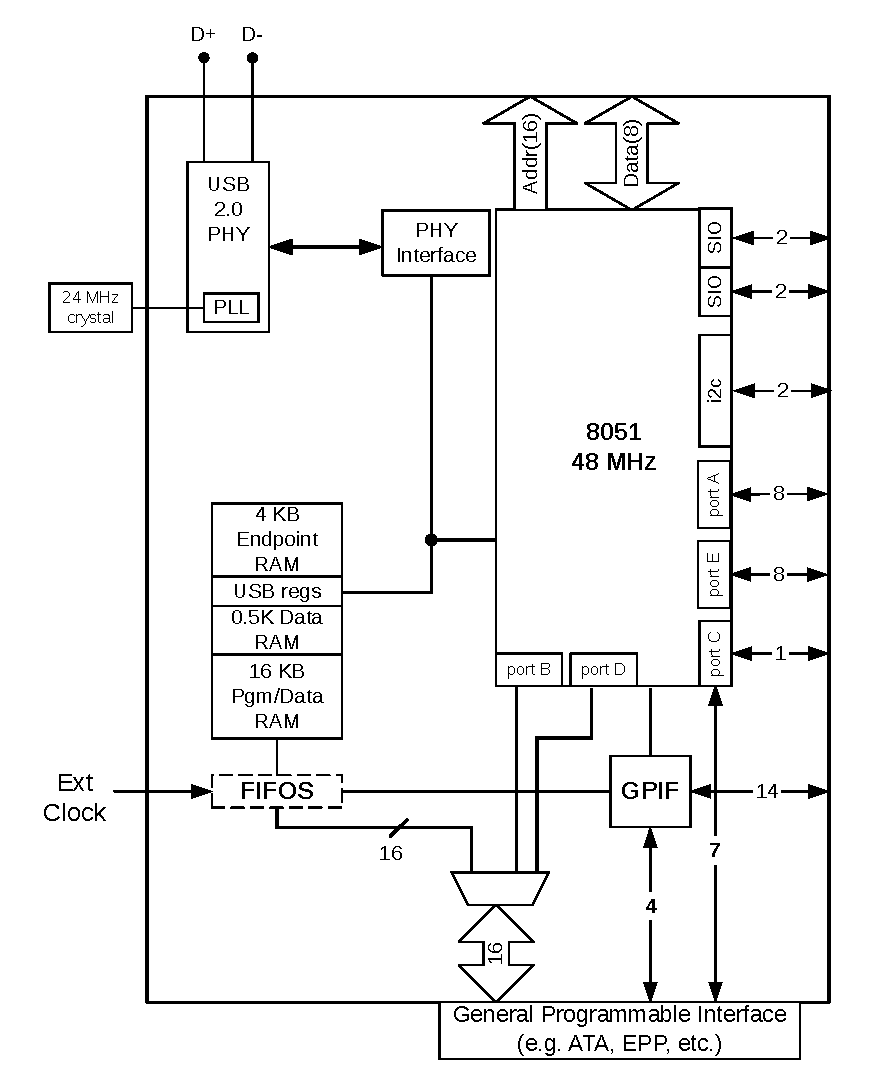
\includegraphics[width=.55\textwidth]{arq.eps}
		%TODO Meter la referencia
		\caption{Arquitectura FX2LP} 
		\label{arqEzUSB}
	\end{figure}

	Esta arquitectura permite al usuario trasmitir datos desde y hacia el anfitrión a través del  mismo puerto USB, o bien via RS-232. A la hora de comunicarse con sistemas periféricos se puede aprovechar el puerto $I^2C$, la interfaz de propósito general o las memorias FIFO en modo esclavo que puede ser conectada a un sistema maestro. Esto brinda muchas alternativas, desde la conexión a puertos estandar, como ser ATA, PCMCIA o EPP, o también la conexión de dispositivos tales como DSP's y FPGA's.\\
	
	La comunicación USB se realiza a través del transceptor, unido al MIS. Como se observa en la Figura \ref{usbxcvr}, el usuario, a fin de intercambiar datos, solo debe colocar o extraer los datos de registros destinados a tal fin y modificar las banderas de handshaking, que en la figura se observan como ACK (abreviación del ingles {\it acknowledge}, que significa reconocer, aceptar o agradecer), que indican si el sistema está disponible, si los datos fueron colocados o leídos, dependiendo el caso tratado. El MIS y el transceptor USB se encargan de empaquetar, enviar, recibir y desempaquetar toda la información, así como leer los tokens que emite el host, calcular y corroborar los códigos cíclicos de detección de errores y todo lo relacionado al protocolo en sí.\\
	
	\begin{figure}[h]
		\centering
		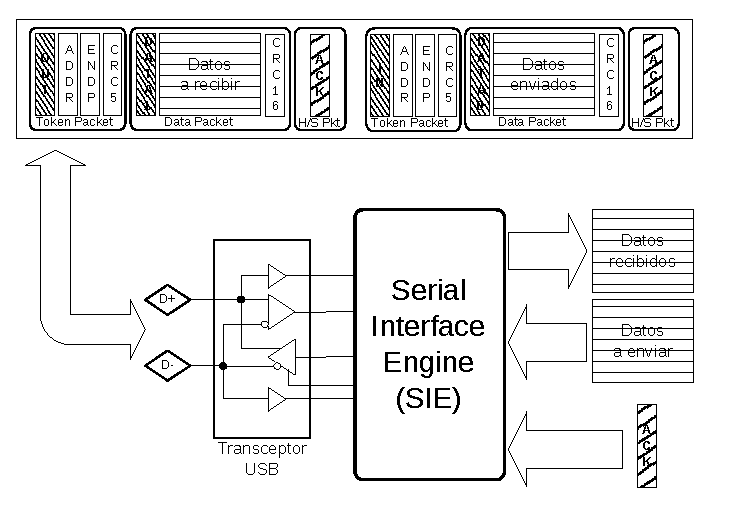
\includegraphics[width=.65\textwidth]{usbxcvr}
		\caption{Implementación del enlace USB realizado por el EZ-USB}
		\label{usbxcvr}
	\end{figure}
	
	El esquema de bus permite utilizar el microcontrolador 8051 para procesar datos, hacer control de errores, empaquetar datos de una forma particular, generar datos nuevos, entre otras, o bien, simplemente enviar datos desde un periférico de forma directa al MIS y luego transmitirlos a la PC por la tubería USB.\\
	
	Para este trabajo final, se configuró el funcionamiento del EZ-USB en modo esclavo, conectando al maestro, el FPGA, a la memoria FIFO destinada para tal fin.\\
	
		\subsection*{Memoria FIFO}
		Al poseer el sistema un MIS, que es un serializador de datos, el sistema usa la memoria FIFO como buffer.%la memoria FIFO de 4kB es usada por el sistema como buffer.
		Se conecta de forma directa a los periféricos y es configurable, lo que permite al usuario disponer del espacio conforme requiera las necesidades de ancho de banda para los sistemas diseñados, evitando así las congestiones en casos de mucho flujo de datos. En el otro extremo, puede ser conectada al tubo USB o al microcontrolador, dirigiendo los datos directamente a la PC o realizando alguna acción sobre ellos antes de enviarlos, respectivamente. Cada uno de estos modos son configurables de forma independiente tanto para los paquetes entrantes como salientes.\\
		
		En la Figura \ref{modesfifo} se grafica lo anterior. Cypress denomina MODO AUTO ENTRADA a los datos que se dirigen desde un periférico hacia anfitrión, de forma directa sin pasar por el microcontrolador. De forma análoga, los datos que salen del anfitrión y no pasan por el 8051, lo hacen en MODO AUTO SALIDA. Cuando los datos pasan por el microcontrolador, se utiliza el MODO MANUAL. Cabe notar que los modos de ENTRADA o SALIDA poseen como referencia el anfitrión debido al carácter central que posee éste en la arquitectura USB.\\
		
		\begin{figure}
			\centering
			\includegraphics[width = 0.6\textwidth]{esquemafifo}
			\caption{Modos de conexión de la memoria FIFO, el microntrolador y el MIS}
			\label{modesfifo}
		\end{figure}
		
		El sistema FX2LP permite configurar los buffers conforme la se ve en la Figura \ref{epconfigs}. Cada buffer tiene una dirección de memoria asignada y corresponde a cada uno de los extremos posibles. Es de destacar que en cualquiera de las configuraciones posibles, se tiene al menos dos buffers. Los diseñadores del integrado pensaron esto como una solución a la congestión. Para ello, los buffers se pueden configurar duplicados, triplicados o cuadruplicados, dependiendo de las necesidades. Luego, el sistema de forma automática se encarga de permutar los buffers, reasignando los espacios de memoria al lugar físico del circuito donde se puedan almacenar nuevos datos, de forma tal que no queden datos retenidos en el dispositivo maestro. Cómo se detallará más adelante, para este trabajo se configuraron dos extremos como el modo 11 de la Figura \ref{epconfigs}, es decir, un extremo con 3 buffers de 1024 bytes y otro con 2 buffers de 512 bytes.\\
		
		Los buffers pueden ser conectados directa hacia el MIS para realizar una comunicación automática entre la PC y los periféricos, estableciendo una cantidad umbral de datos que, cuando se rebasa, envía los datos hacia la PC; o bien se puede acceder a ellos desde el microcontrolador, leer, chequear y/o editar los datos antes de enviar hacia la PC o los periféricos.\\
			
		\begin{figure}[h]
			\centering
			\includegraphics[width=0.6\textwidth]{bufconf}
			\caption{Configuraciones admitidas para los buffers de periféricos}
			\label{epconfigs}
		\end{figure}